\chapter{PAM modulator and demodulator}

PAM modulation is done by multiplying a square wave by message signal.
\textit{The minimum amplitude of square wave should be 0}, which can be either constructed by \texttt{square} or \texttt{sin} function:
\begin{itemize}
	\item \texttt{sin(2 * pi * fc * t) > 0}
	\item \texttt{square(2 * pi * fc * t) > 0}
\end{itemize}

% \section{Demodulation}
% Demodulation can be done in 2 ways: cumulatI'vesummer and low pass filter.
% \subsection{Low pass filter}

% For perfect integration: $RC > 15T$ where $T=1/f$

% If the frequency of clock is f = 1 KHz

% $$RC > \frac{15}{1kHz}$$

% Let $C = 1\uf$, then 

% \begin{align*}
% 	R &> \frac{15}{1kHz * 1\uf} \\
% 	R &> 1.5k\ohm
% \end{align*}

% in fact any value of $R > 1.5k\ohm$ will work. But more the value of $R$, more will be the attenuation
% \subsection{CumulatI'vesummer}

Demodulation is done by a passing PAM wave to low pass filter with cut off frequency slightly higher than highest frequency in the message signal.
\section*{Program}
Here message is $m(t) = 0.5\sin(2\pi f_m t) + \sin(6\pi f_m t)$

\importMLCode{code/pam_exp.m}

\begin{figure}[!ht]
	\centering
	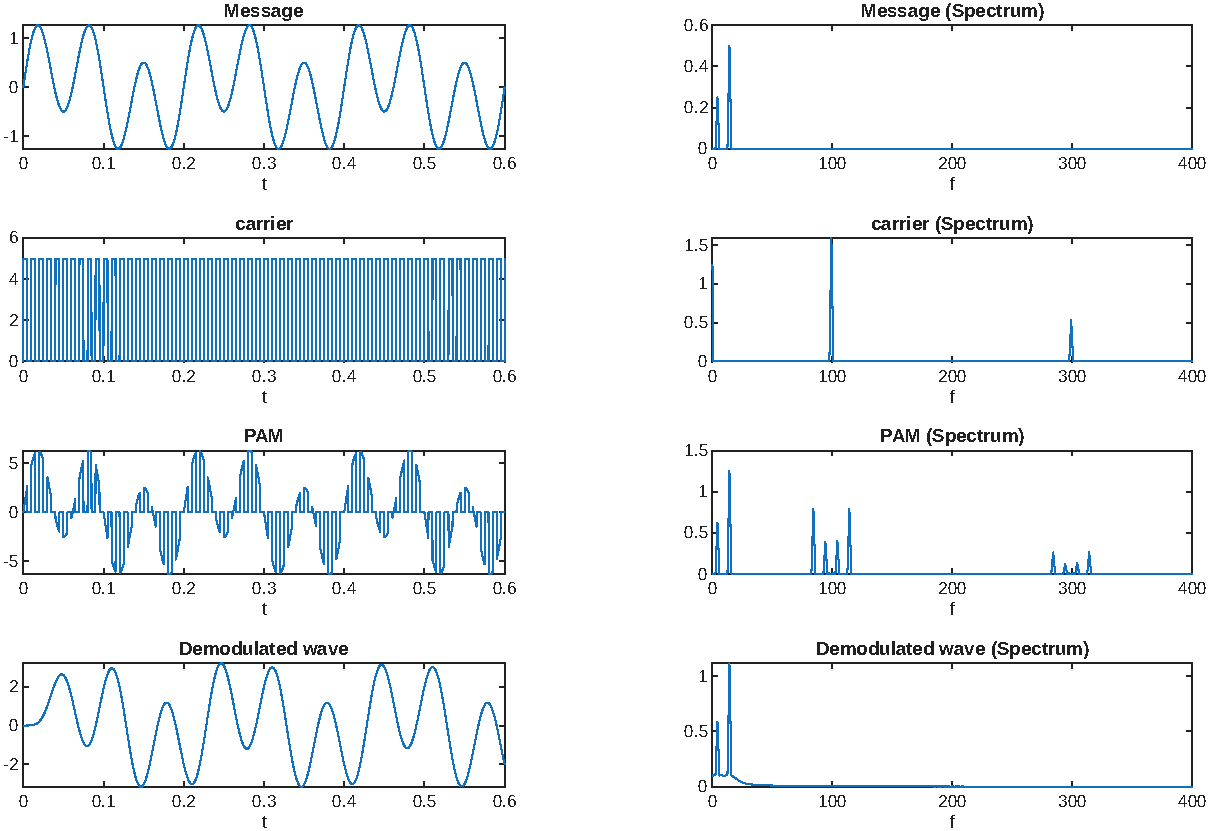
\includegraphics[width=\textwidth]{img/pam.pdf}
\end{figure}

\pagebreak